\chapter{Results and Analyses} \label{chap:result}

This chapter is dedicated not only to give an overview of the results of the simulation, but also to analyse the given results within certain parameters. This chapter is, in essence, where the problem statement in section \vref{sec: Problem Statement} can finally be answered.

The results shown and analysed are all based on the same seed (the seed being 808420), making it possible to reproduce the results both with and without contact tracing. 

We have created our results by simulating 1,000 drops with and without contact tracing enabled. In the following sections the two simulations will be compared to each other. This is done by plotting the data found in Appendix \ref{Appendix:Data} onto graphs. These then visualise the differences and can be analysed. 

\section{Results from the Simulation}

To create a baseline for the remainder of the results of the simulation results, we will first outline and analyse results from the simulation, with the standard parameters for the virus and contact tracing, which we have defined and described in the previous chapter in section \ref{subsec:Data in Sim}.

All parameters and their accompanying values can be seen in the table \vref{Parameter table} below:

\label{Parameter table}
\begin{center}

\begin{tabularx}{0.9\textwidth} { 
  | >{\raggedright\arraybackslash}X 
  | >{\raggedright\arraybackslash}X 
  | >{\raggedright\arraybackslash}X
  | >{\raggedright\arraybackslash}X| }

 \hline
 \multicolumn{2}{|c|}{Parameters and their value} \\
 \hline
  Population Size & 12,500 persons\\
 \hline
  Average contacts & 10 persons\\
 \hline
  Quarantine period & 14 days \\
 \hline
  Reproductive number & 2.63 \\
 \hline
  Average infection period & 10 days \\
 \hline
  Incubation period & 3 - 10 days\\
 \hline
  Asymptomatic period & 1 - 10 days \\
 \hline
  Contact tracing start time & day 30 \\
 \hline
  Traceable contacts & 5 - 20 persons \\
 
 
\hline
\end{tabularx}

\end{center}

This table will be referenced several times in this chapter.

\begin{figure}[H]
    \centering
    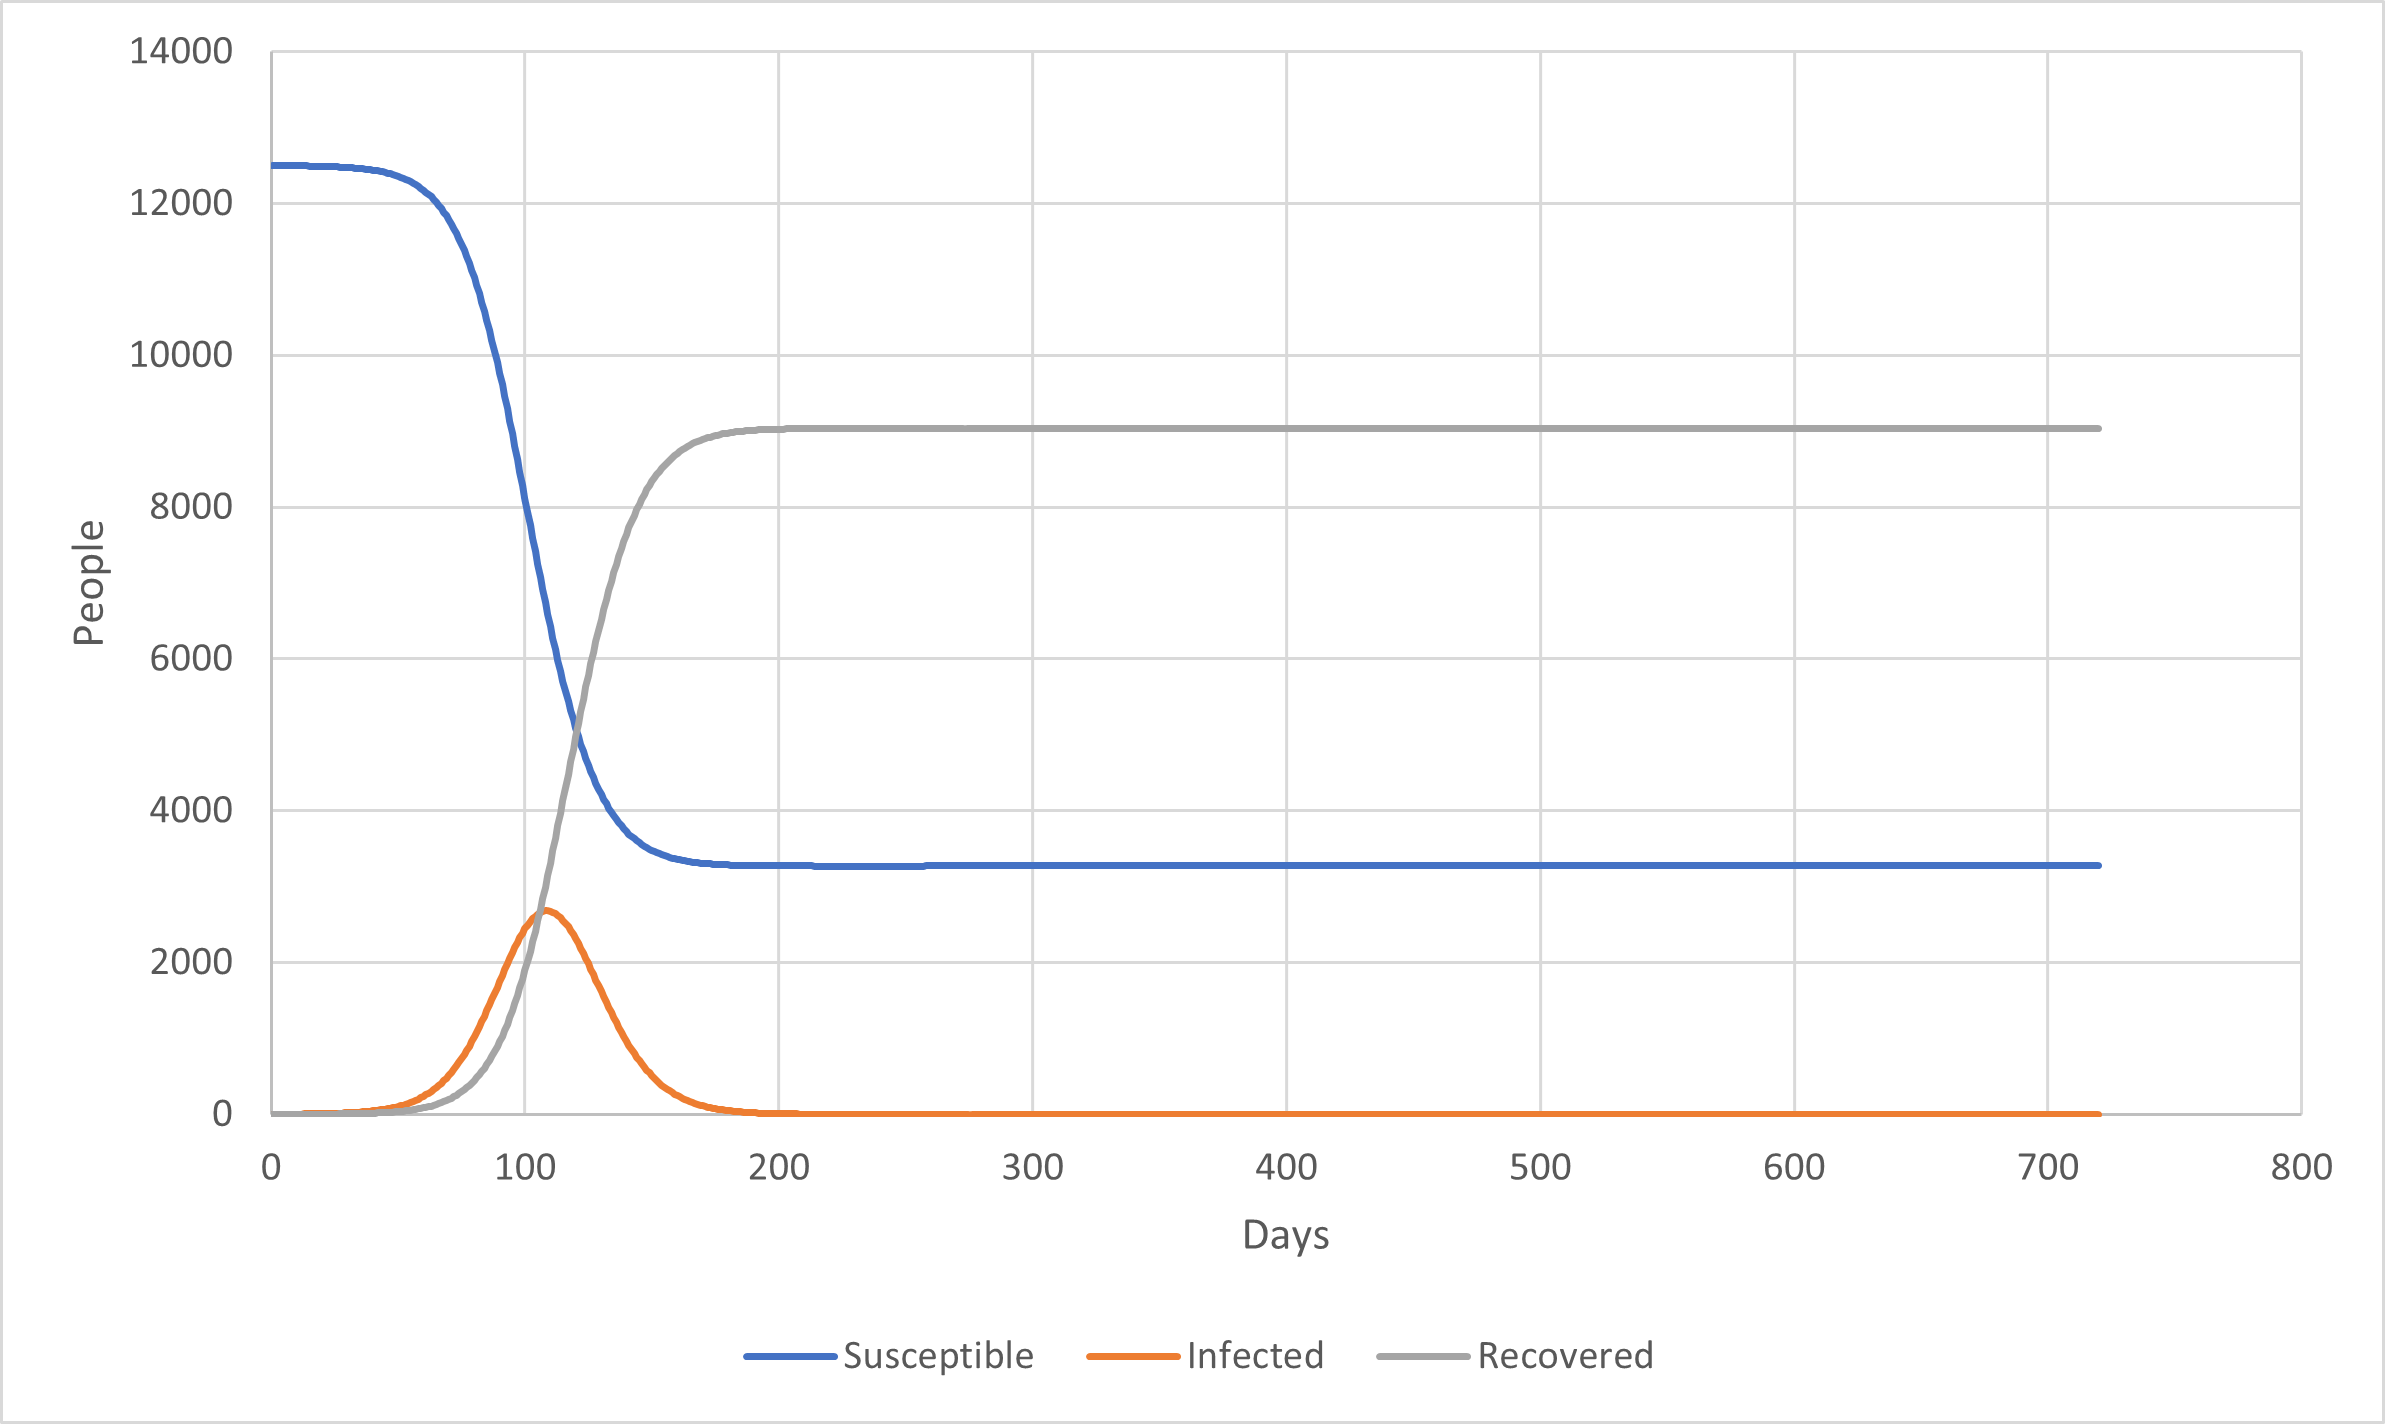
\includegraphics[width=0.75\textwidth]{0_billeder/Sim_CT_OFF.png}
    \caption{Graph of susceptible, infected and recovered plotted against days, from simulation without contact tracing}
    \label{fig:Sim_CT_OFF-1}
\end{figure}

Figure \ref{fig:Sim_CT_OFF-1} is a graph containing the averages from a 1000 drops, showing how individuals in the population change status throughout the time frame with no contact tracing to mitigate the spread.

As is shown in \ref{fig:Sim_CT_OFF-1}, the infection peaks and dies out rather quickly (within the first 200 days). By the end of the time frame, some people remain uninfected (susceptible), while the majority of the population have recovered. This is quite different from figure \ref{fig:Sim_CT_ON-1}, as shown below.

\begin{figure}[H]
    \centering
    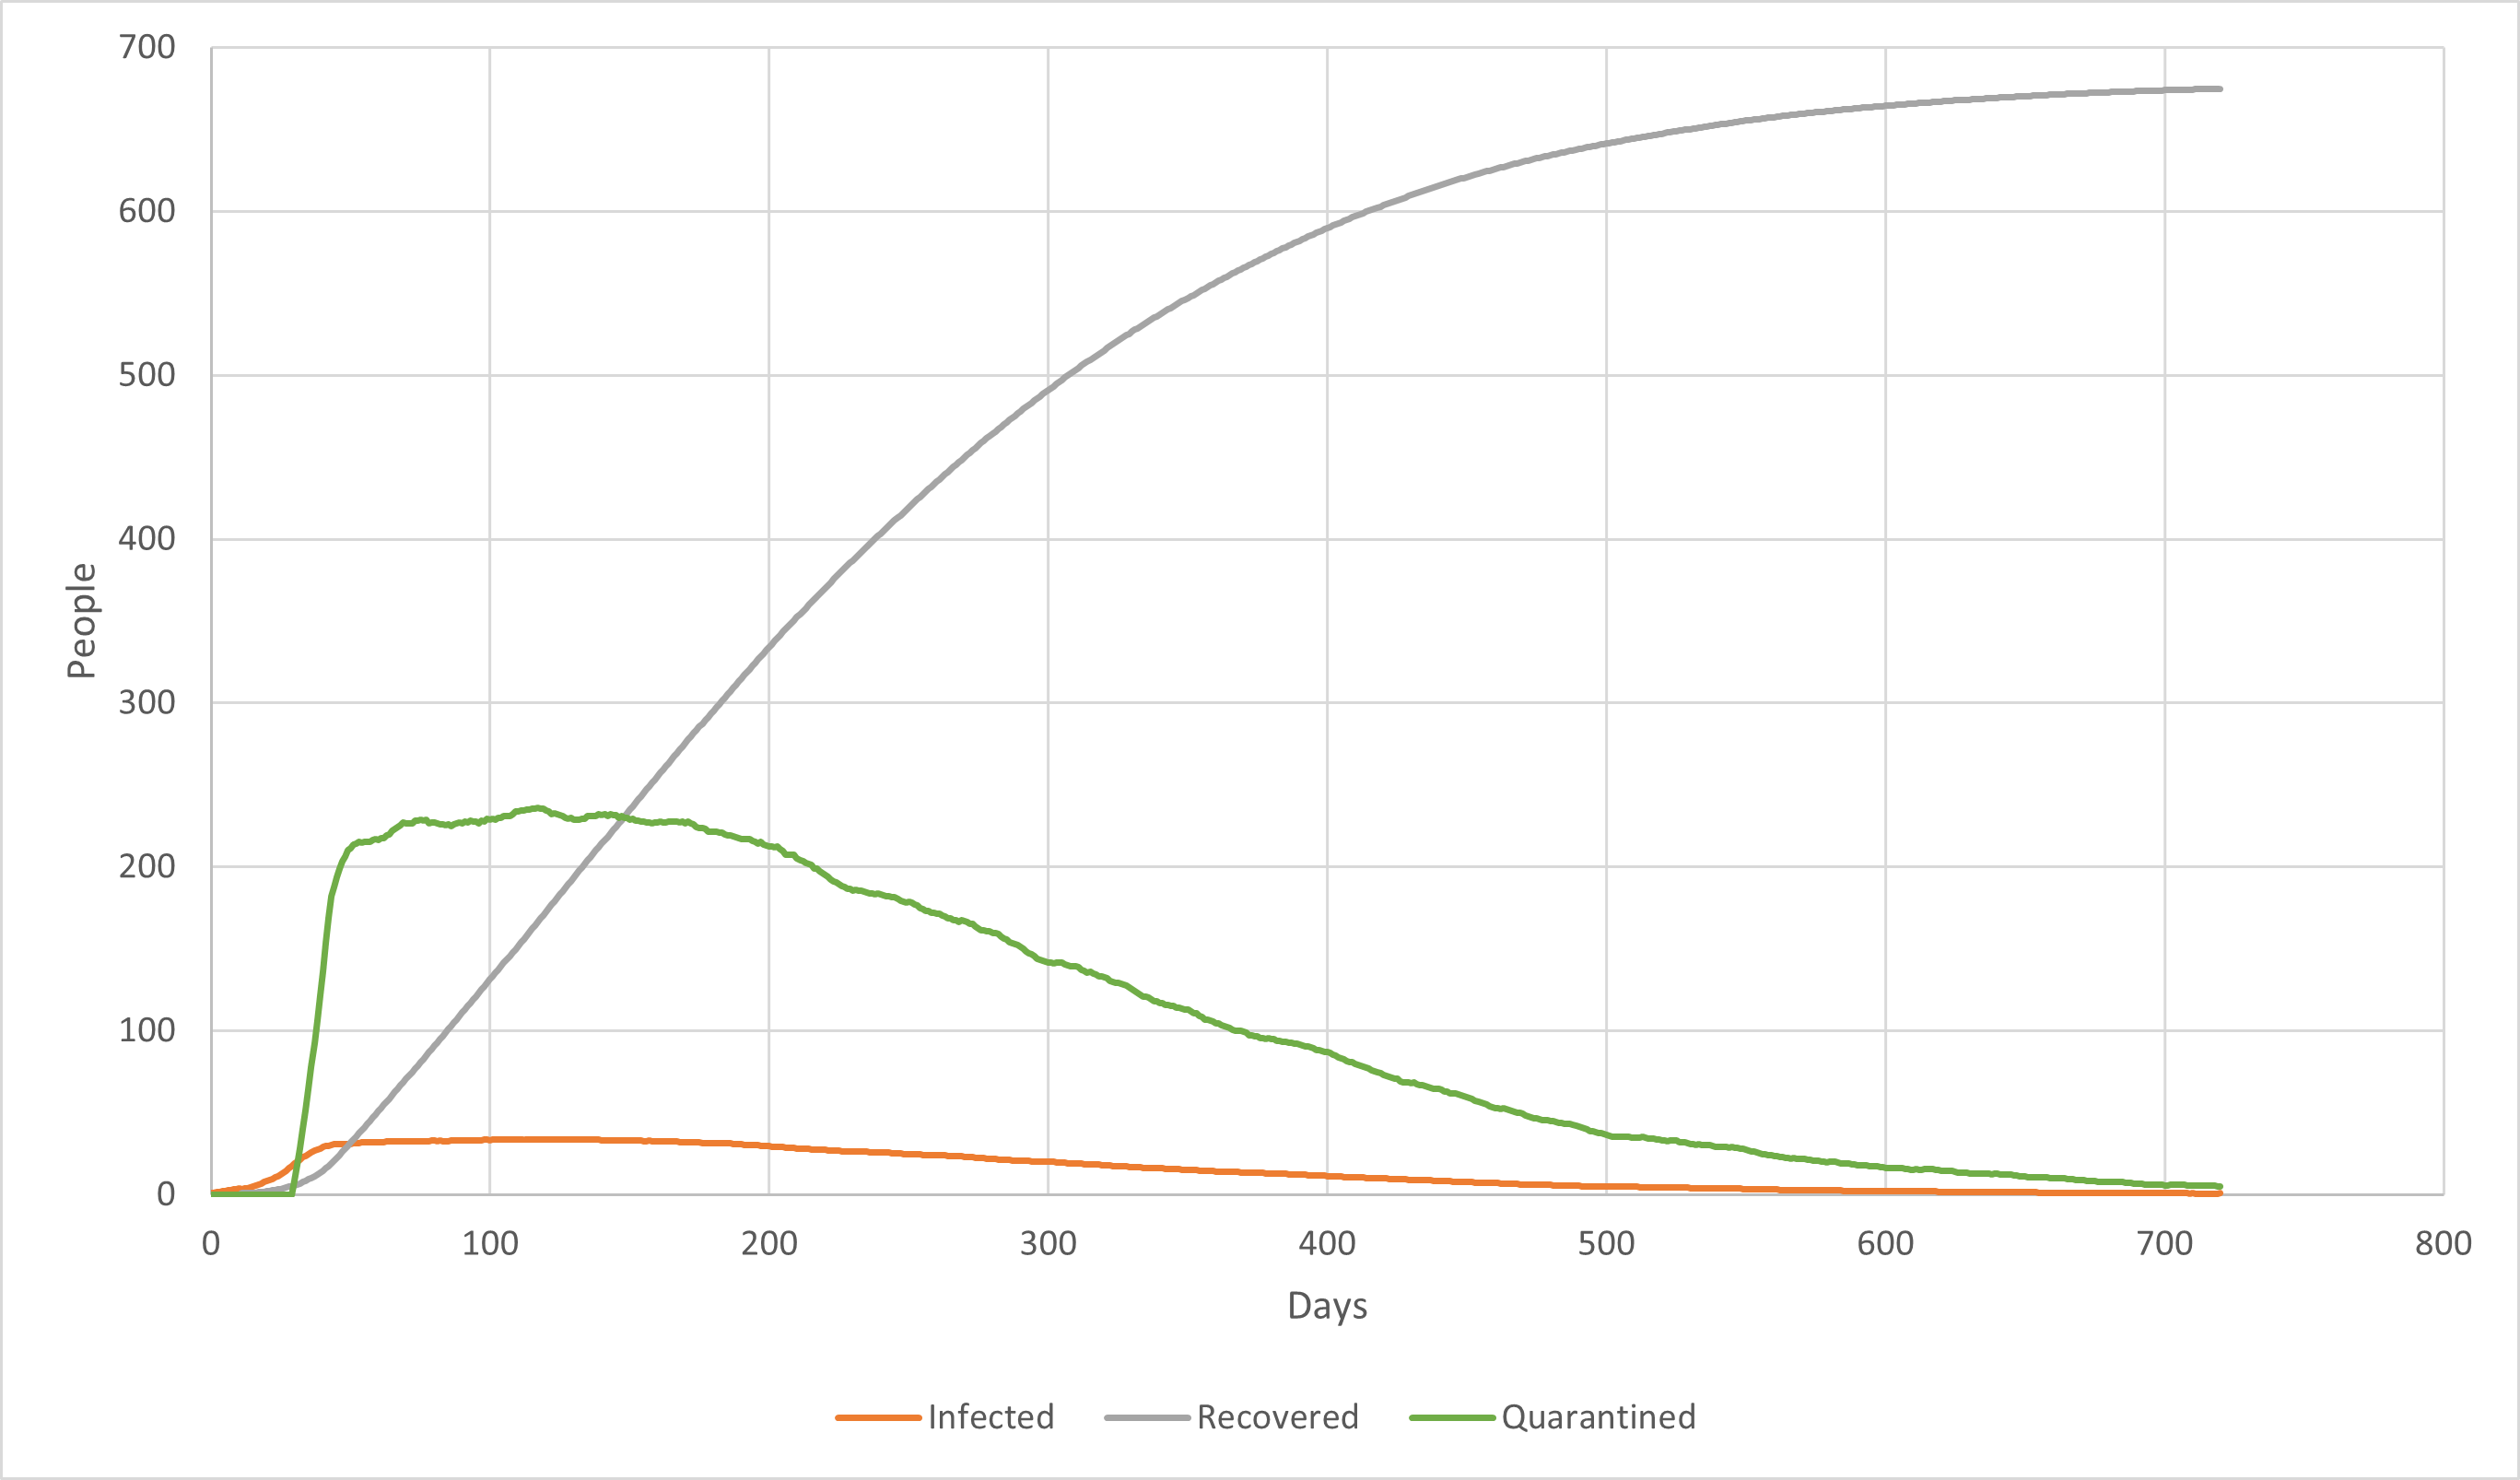
\includegraphics[width=0.75\textwidth]{0_billeder/Sim_CT_ON.png}
    \caption{Graph of quarantined, infected and recovered plotted against days, from simulation with contact tracing}
    \label{fig:Sim_CT_ON-1}
\end{figure}

In figure \ref{fig:Sim_CT_ON-1}, contact tracing has been enabled alongside quarantine. As is shown, this lengthens the infection period for the population as a whole, but greatly diminishes the number of infections across the population. 

Whereas there are about 900 recovered in the simulation run with no contact tracing (figure \ref{fig:Sim_CT_OFF-1}), there are under 700 recovered in the simulation run with contact tracing (figure \ref{fig:Sim_CT_ON-1}). This shows that contact tracing not only lowers the risk of infection to the individual person but also indicates a decrease in total amount of deceased. 

It should also be noted that while contact tracing is activated, quarantine is similarly activated. In a similar vein, as is shown in figure \ref{Fig:covidInfGraphs} below, there is a correlation between contact tracing, quarantine and deaths.

\begin{figure}[H]
 \centering
  \begin{subfigure}{.485\textwidth}
    \centering
    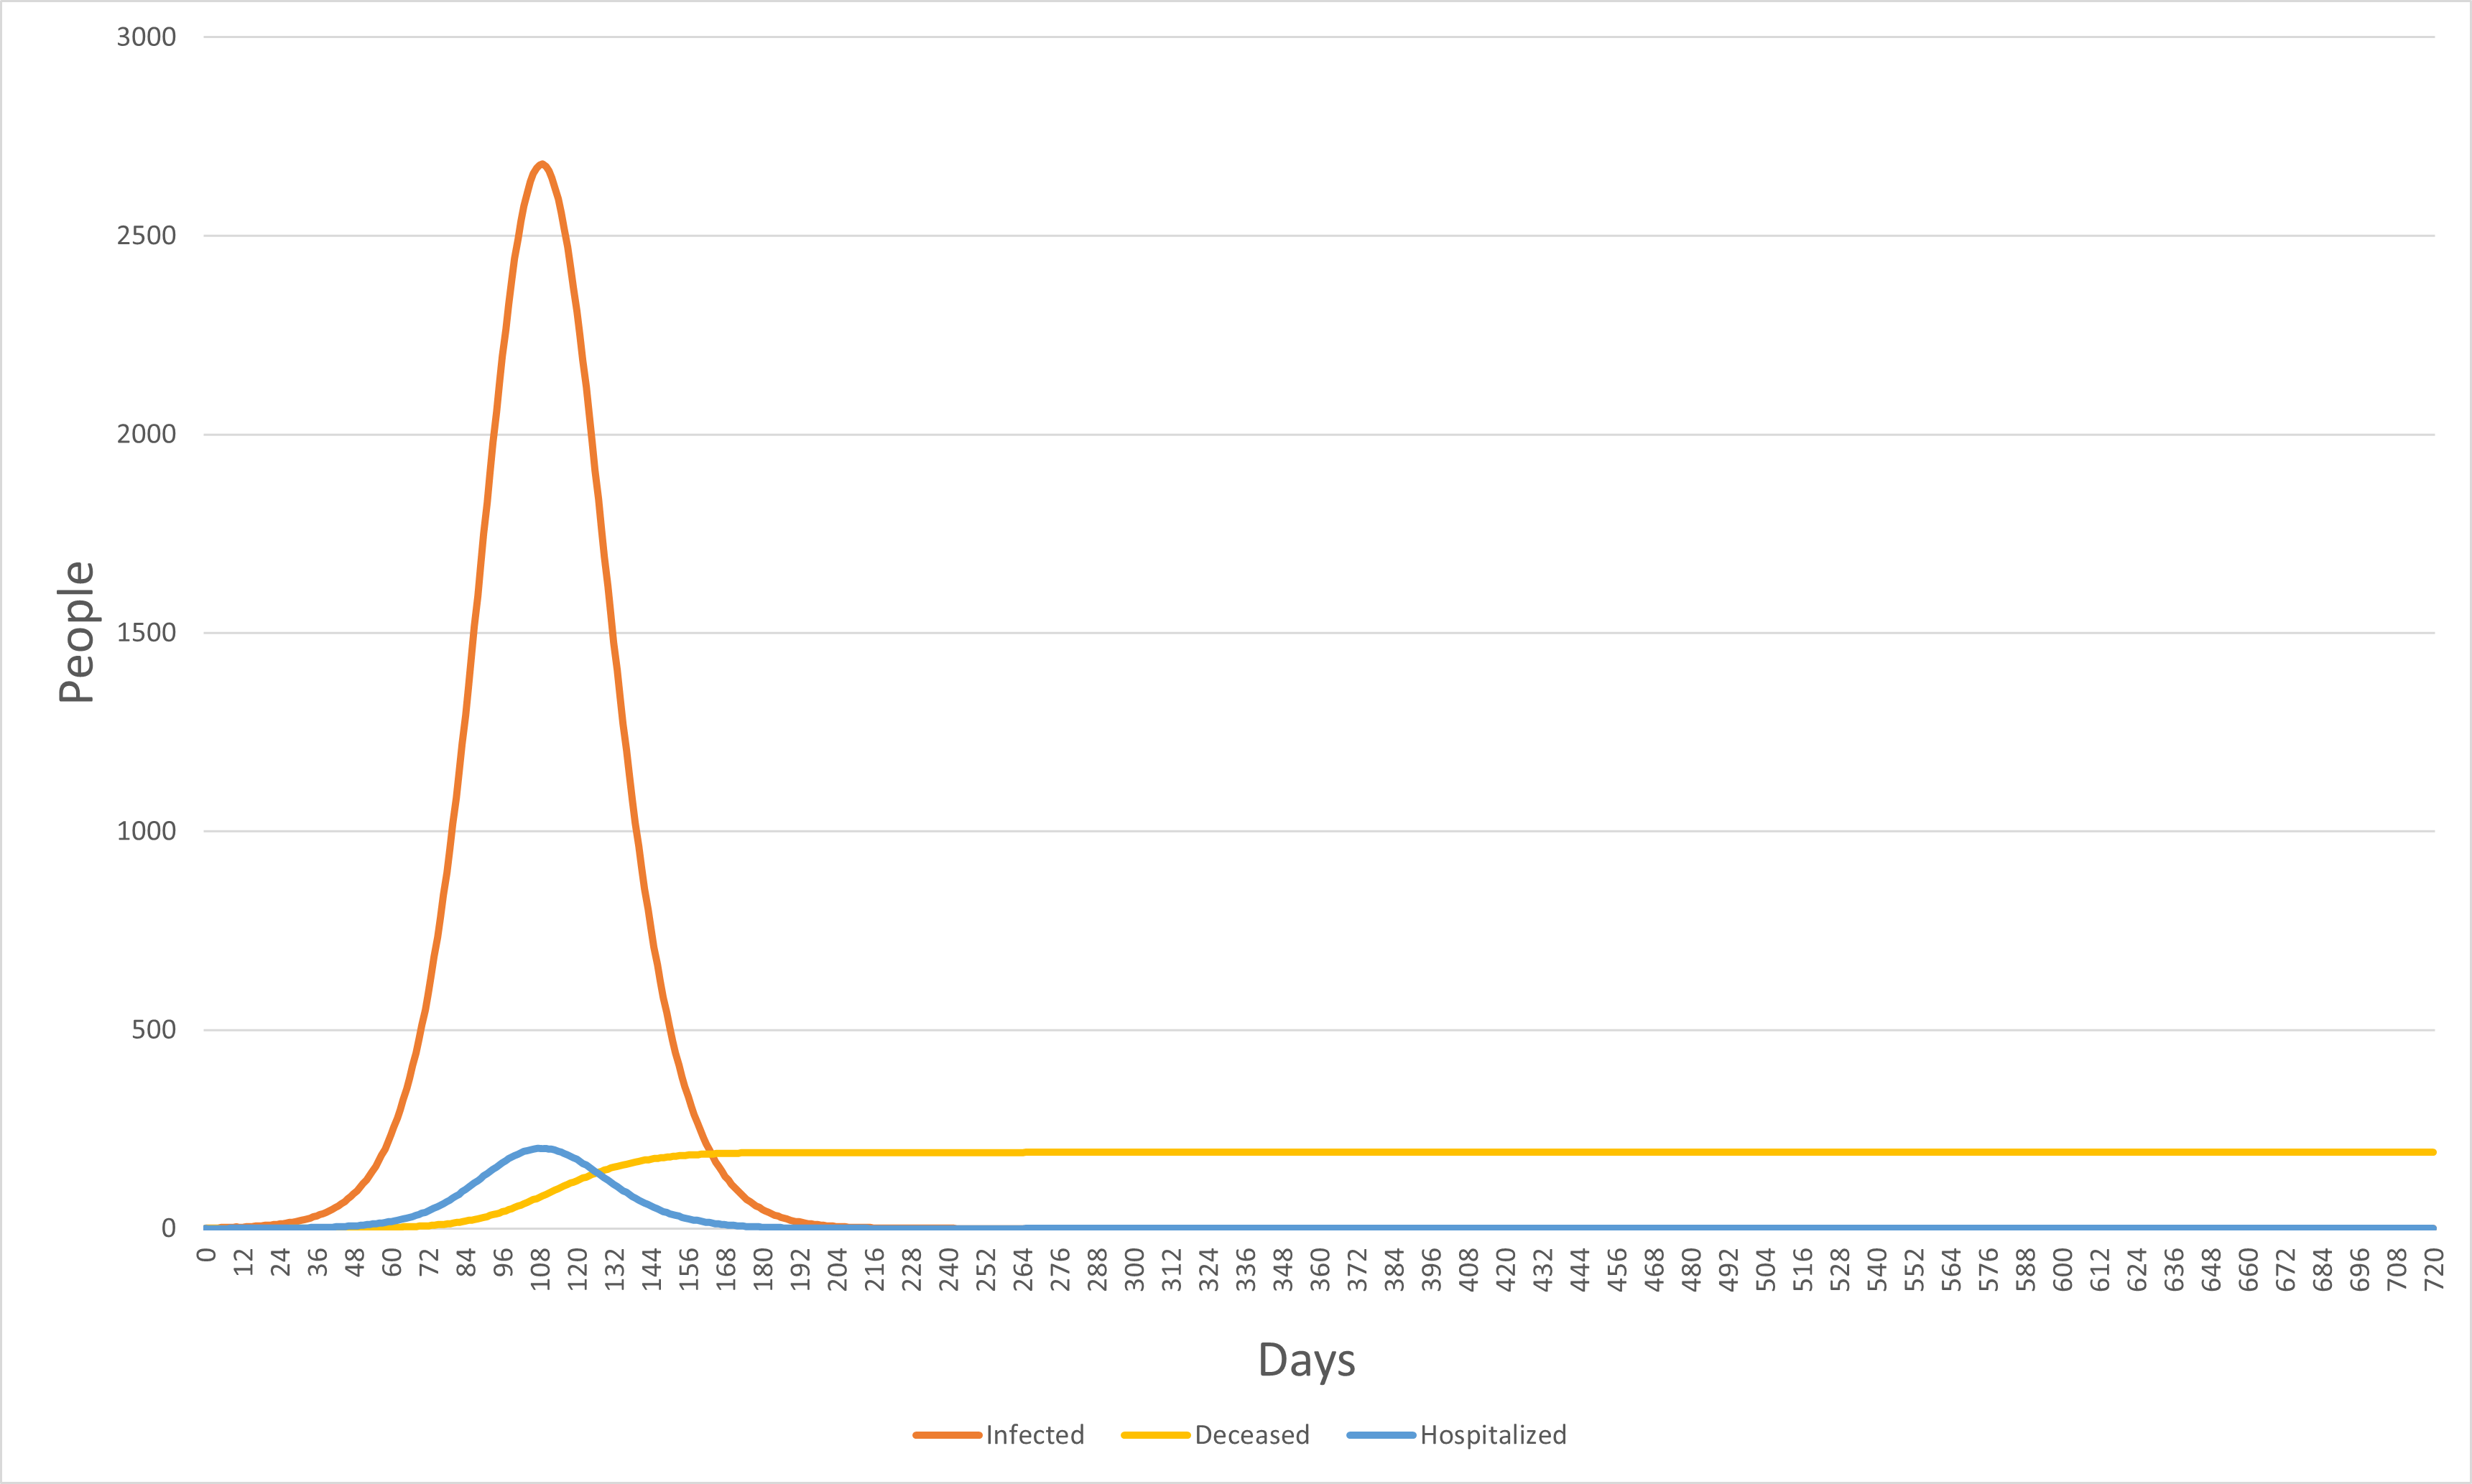
\includegraphics[width=.95\linewidth]{0_billeder/covidInfectionGraphA.png}
    \caption{With contact tracing}
    \label{Subfig:covidInfGraphA}
  \end{subfigure}
  \begin{subfigure}{.485\textwidth}
    \centering
    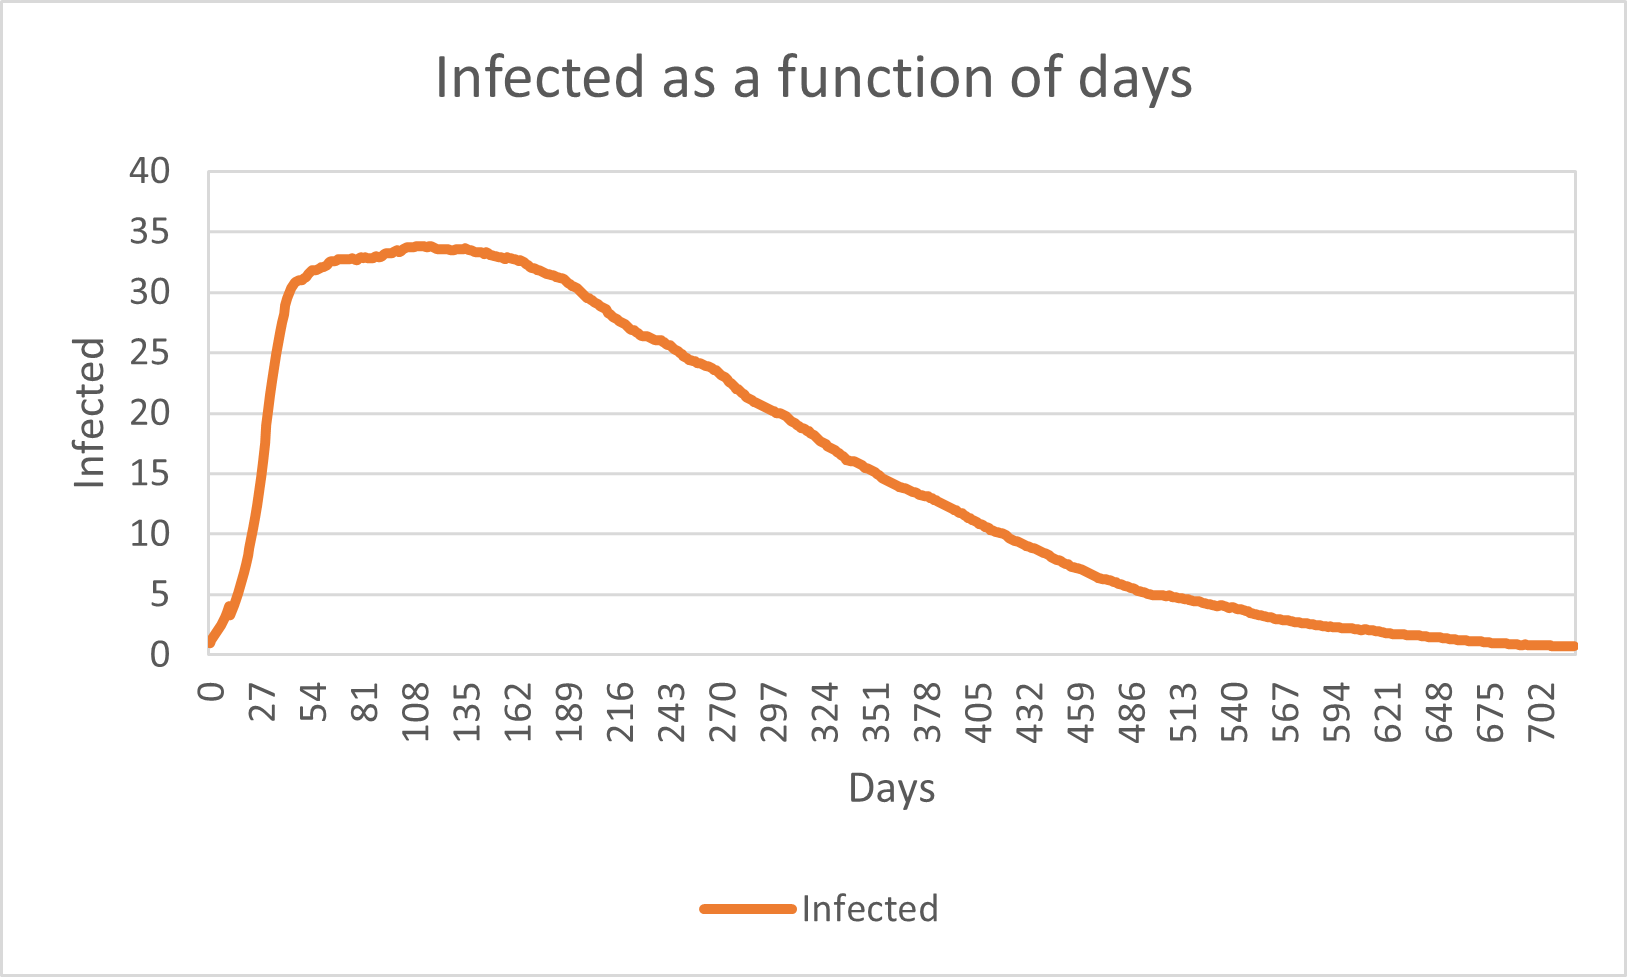
\includegraphics[width=.95\linewidth]{0_billeder/covidInfectionGraphB.png}
    \caption{Without contact tracing}
    \label{Subfig:covidInfGraphB}
  \end{subfigure}
 \caption{Infection graphs with and without contact tracing.}
 \label{Fig:covidInfGraphs}
\end{figure}

Figure \ref{Fig:covidInfGraphs} is a graph of infection, as a function of days, both with and without contact tracing enabled. Before explaining the graphs, it is important to note that the data used is an average of 1,000 drops.

In the first graph with contact tracing disabled, we see that the number of infected people is rising rapidly to its peak which is around 2750 people infected on day 112. After the peak, the number of infected people quickly drops to 0 again around day 190 and does not change further.

In the second graph, which is with contact tracing enabled, the number of infected also rises rapidly, but it does not reach the same levels as in the first graph. The maximum number of infected in the second graph is around 33 on day 140. After it has peaked, it slowly decreases, reaching 0 cases of infection around day 720.

Comparing the two, it is clear that contact tracing and quarantine is a very effective tool in fighting COVID-19. With contact tracing disabled, the number of infections peaks at 2750 people, whereas with contact tracing enabled, it peaks at only 33 people. That corresponds to only 1.2\% of the first graph's peak.

It can also be noted that this decrease in infections has a major impact on the mortality and hospitalisation rates in the simulation. The peak in figure \ref{Subfig:covidInfGraphA} is about 202 for hospitalisation and about 192 for deceased. This is in stark contrast to the peaks on figure \ref{Subfig:covidInfGraphB} which is circa 2.5 for hospitalisation and approximately 13.8 for deceased which is a decrease of over 90\% for both.

It can therefore be concluded that including contact tracing and quarantine minimises mortality rates and also lengthens the infection period for the population.


